\documentclass[12pt]{extarticle}
\usepackage[utf8]{inputenc}
\usepackage{import}
\usepackage{cite}
\usepackage{graphicx}


\title{An Empirical Discussion on Golden Ratio, $\Phi$}
\author{Nesar Ul Alam}
\begin{document}
\begin{figure}[h]
\centering

\includegraphics[width=16.03cm,height=6.98cm]{image1.jpeg}
\end{figure}
\textbf{ }

\begin{center}\textbf{SOEN 6481}\end{center}

\begin{center}\textbf{Software Requirement Specifications}
\end{center}

\begin{center}\textbf{Golden Ratio}\end{center}



\begin{center}\textbf{Author - Nesar Ul Alam}\end{center}

\begin{center}\textbf{Student ID - 40105752}\end{center}




\newpage
\tableofcontents

\newpage
\section{Abstract}
Golden Ratio is denoted by the Greek letter Phi ($\phi$), the value is 1.6180339887 approximately.It has unique and mystifying properties,researchers
and mathematicians have been studied about the Golden Ratio.Renaissance architects,
artists and designers also studied on this interesting topic, documented and employed the Golden section proportions in
eminent works of artifacts, sculptures, paintings and architectures. The Golden Ratio also known as Golden Proportion is considered as the most pleasing
to human visual sensation and not limited to aesthetic beauty but also be found its existence in natural world through the body
proportions of living beings, the growth patterns of many plants, insects and also in the model of enigmatic universe. \cite{geometricalphi}
\newpage

\section{Acknowledgement}
I would like to express my sincere gratitude and appreciation to my Professor Pankaj Kamthan, for providing relevant lecture notes,guidance and suggestions throughout Deliverable 1 for the project.\newline\newline
Moreover, I would also like to thank my group mates who helped me during the course of the project and made this time joyful.
\newpage
\section{Problem 1: Introduction}
Golden Ratio, first depicted and described by Euclid in the golden age of Greek Knowledge, discusses about a fundamental characteristics in the number theory. A number is said to be in a Golden Ratio if their ratio is found to be same as the ratio of their sum to the larger of the two. The Greek letter $\phi$ is used as the symbol of Golden Ratio. The value of $\phi$ is 1.61803398875. The number itself is irrational. The term ``Golden" has been used as it is considered to be aesthetically pleasing and examples of the ratio can be drawn from the nature itself.

In terms of mathematics, the Golden Ratio can be described in many different ways. However, for the sake of simplicity, we must start from the first description of the ratio, as depicted by Euclid, the line segment theory. It goes in this way- 

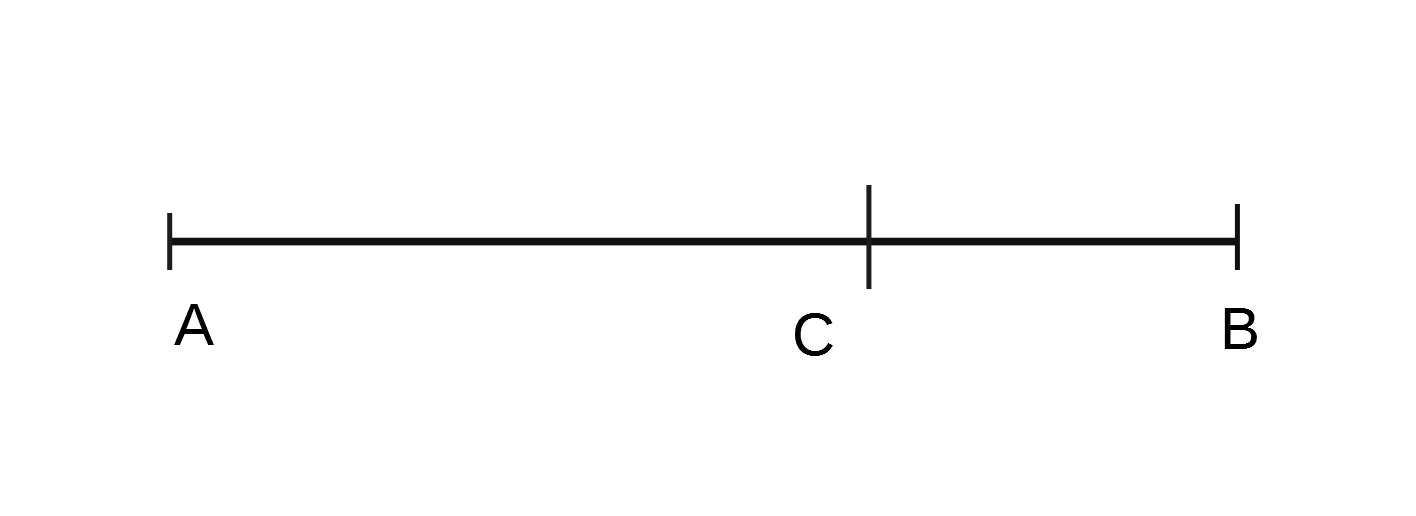
\includegraphics[]{ffUntitled.png}

As can be seen from the image, length of $AB$ is greater than that of $AC$ and $AC$ is greater than $CB$. if $AC$ $:$ $CB$ is equals to $AB$ $:$ $AC$, then we can conclude that the line has been cut in a Golden Ratio. \cite{livio2008golden}. \newline

\newpage
\section{Problem 2:Interview}


\hspace{2cm}      Interviewee- Niloy Eric Costa \newline


Q1. What are you researching on?


A1. I am working on Interactive Data Visualization.\newline

Q2. Are there any other fields in Computer Science or Mathematics you are interested in?

A2. In the field of Mathematics I'm interested in Geometry and Number Systems and in the field of Computer Science I'm interested in Data Visualization, Database Systems and Data Mining.
\newline 


Q3. Have you heard of any irrational constants in Mathematics? 


A3. I have researched on some irrational constants like $\pi$,e,Khinchins Constant (K).
\newline

     Q4. What do you know about Golden Ratio,$\Phi$ ?
     
     
     A4. Well to explain it.Two quantities are in the golden ratio if their ratio is the same as the ratio of their sum to the
larger of the two quantities. For quantities a and b such that $a > b > 0$,
$$(a+b)/a =a/b$$
     \newline

    Q5. Do you know when we celebrate phi day?
    
    
    A5. Haha. Yeah, 18th June.
    \newline
    
    Q6. Phi is named after a Greek sculptor; do you know his name?
    
    
    A6. Yes, Phidias.
    \newline

   Q7. Do you know any other names golden ratio is known by?
   
   
   A7. Yes.It is known by the Golden Mean, Phi, the Divine Section, The Golden Cut, The Golden Proportion, The Divine Proportion, and tau(t).
   \newline
   
   Q8. How do you derive the value of golden ratio? 
   
   
   A8. By using the quadratic equation $x^2-x-1=0$
   \newline
   
   Q9. Can you tell us about any applications of Golden Ratio?
   
   
   A9. The golden ratio is used mostly in the Geometry to create designs that are in proportions and are
pleasing to the eye. It is not used as such in Mathematics directly but even the ratio of consecutive
numbers in fibonacci series are close to the golden ratio.
   \newline

   Q10. Can you describe some uses of Golden Ratio in architecture and art?
   
   
   A10. The Great Pyramids of Gaza, Parthenon in Athens, Michelangelo’s The Creation of Adam on the
ceiling of the Sistine Chapel and Da Vinci’s Mona Lisa are some of the famous examples that use the
Golden Ratio.
   \newline

  Q11. The ancient Egyptians used the golden ratio in their pyramids. At that time,     the golden was known to them by another name, do you know the name?
  
  
  A11. The Sacred Ratio.
  \newline

   Q12. Do you know about any other fields golden ratio is claimed to appear?
   
   
   A12. The golden ratio is claimed to appear in many fields, such as cosmology, theology, arts, architecture, botany and others.
   \newline
   
   Q14.Would you like to include Irrational constants like Golden ratio in the calculator?


A14. Yes. I would prefer it, as I would work with Golden Rectangle in the future.
\newpage
\section{Problem 3: Persona}
\hspace{4.5cm}   \underline{Problem 3}

\begin{figure}[htb!]
  
  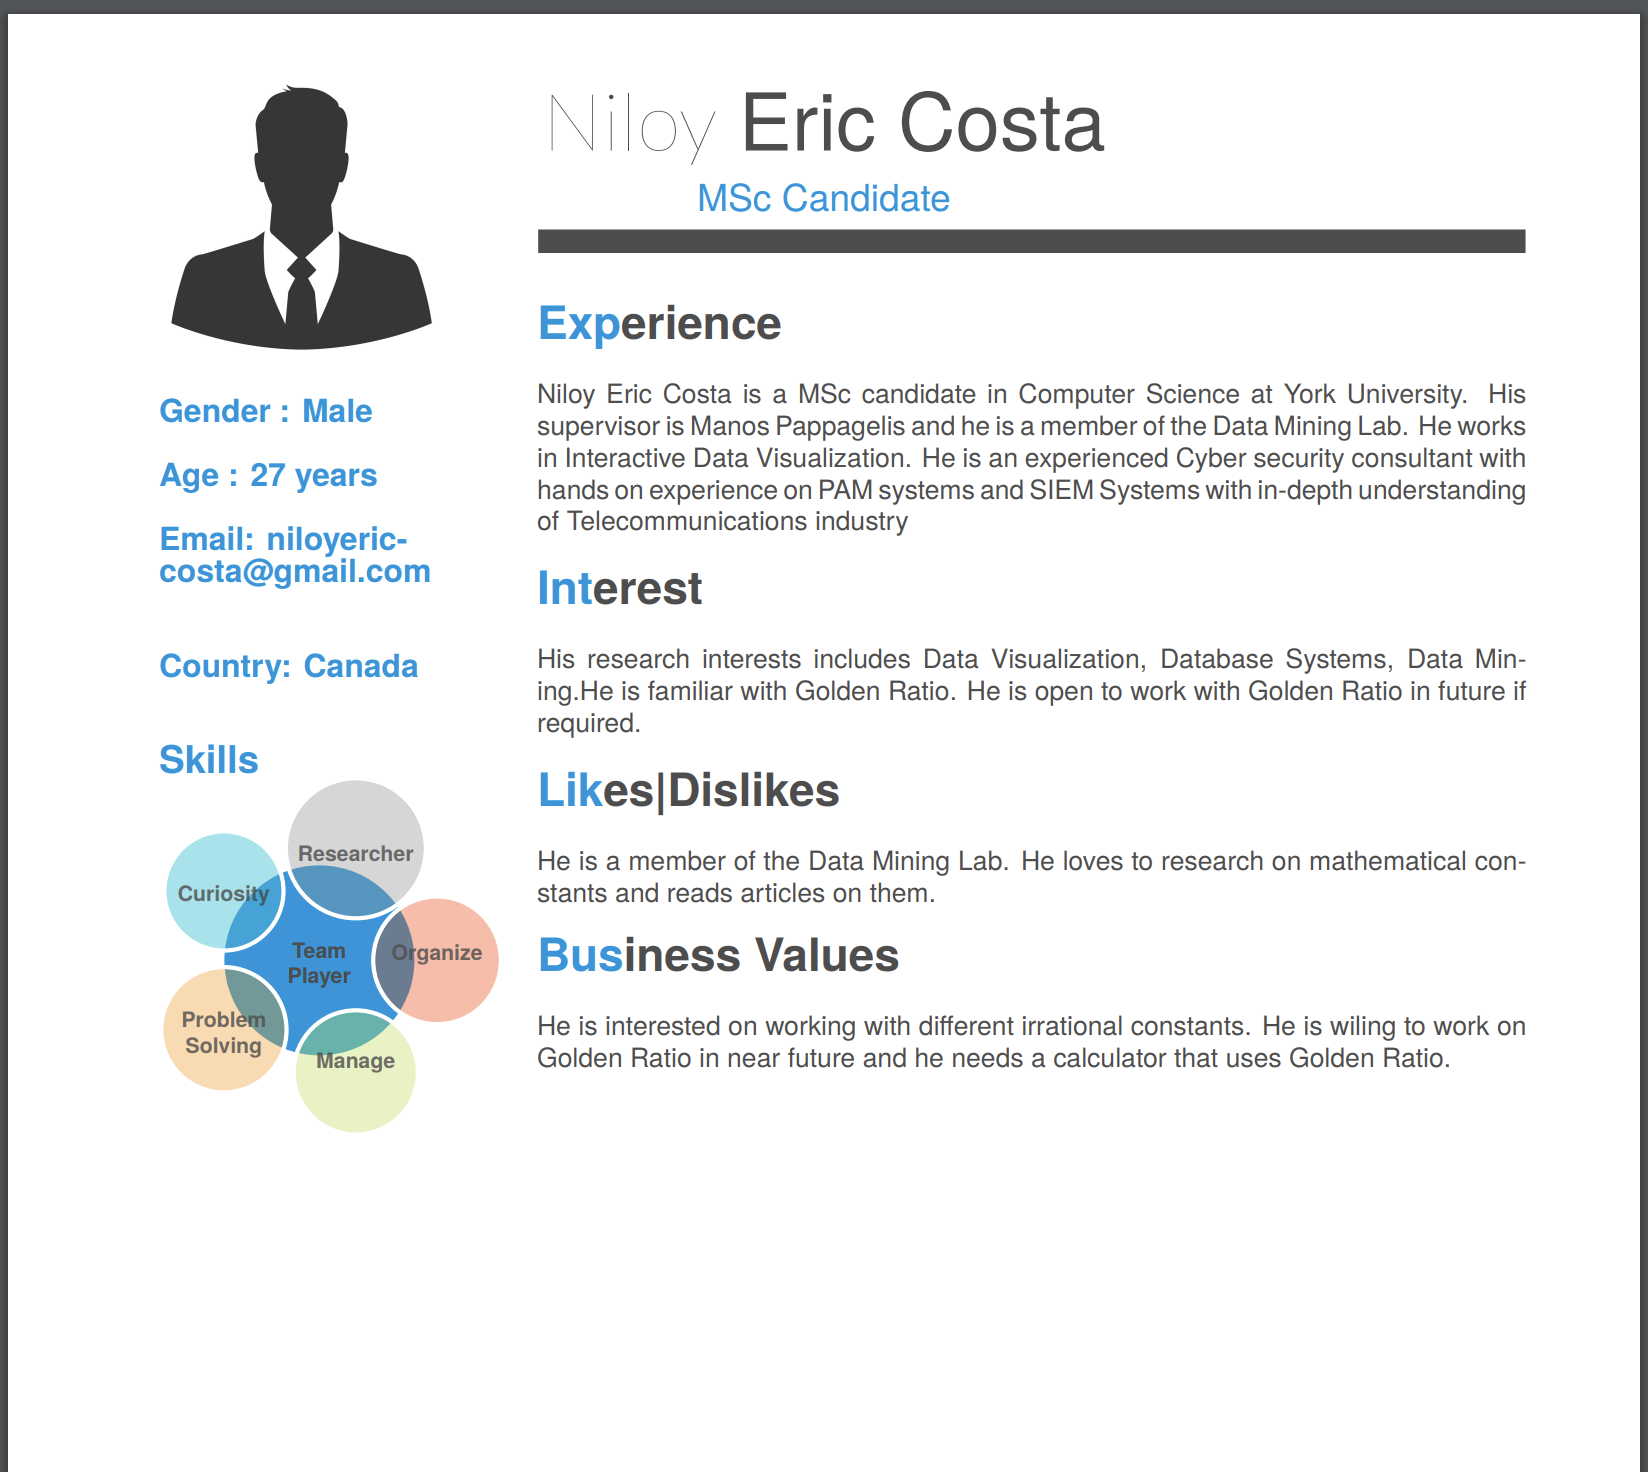
\includegraphics[width=1\textwidth]{niloy.png}
  \centering
  \caption{Persona}
\end{figure}

\newpage
\section{Problem 4: Domain Model}
\begin{figure}[htb!]
  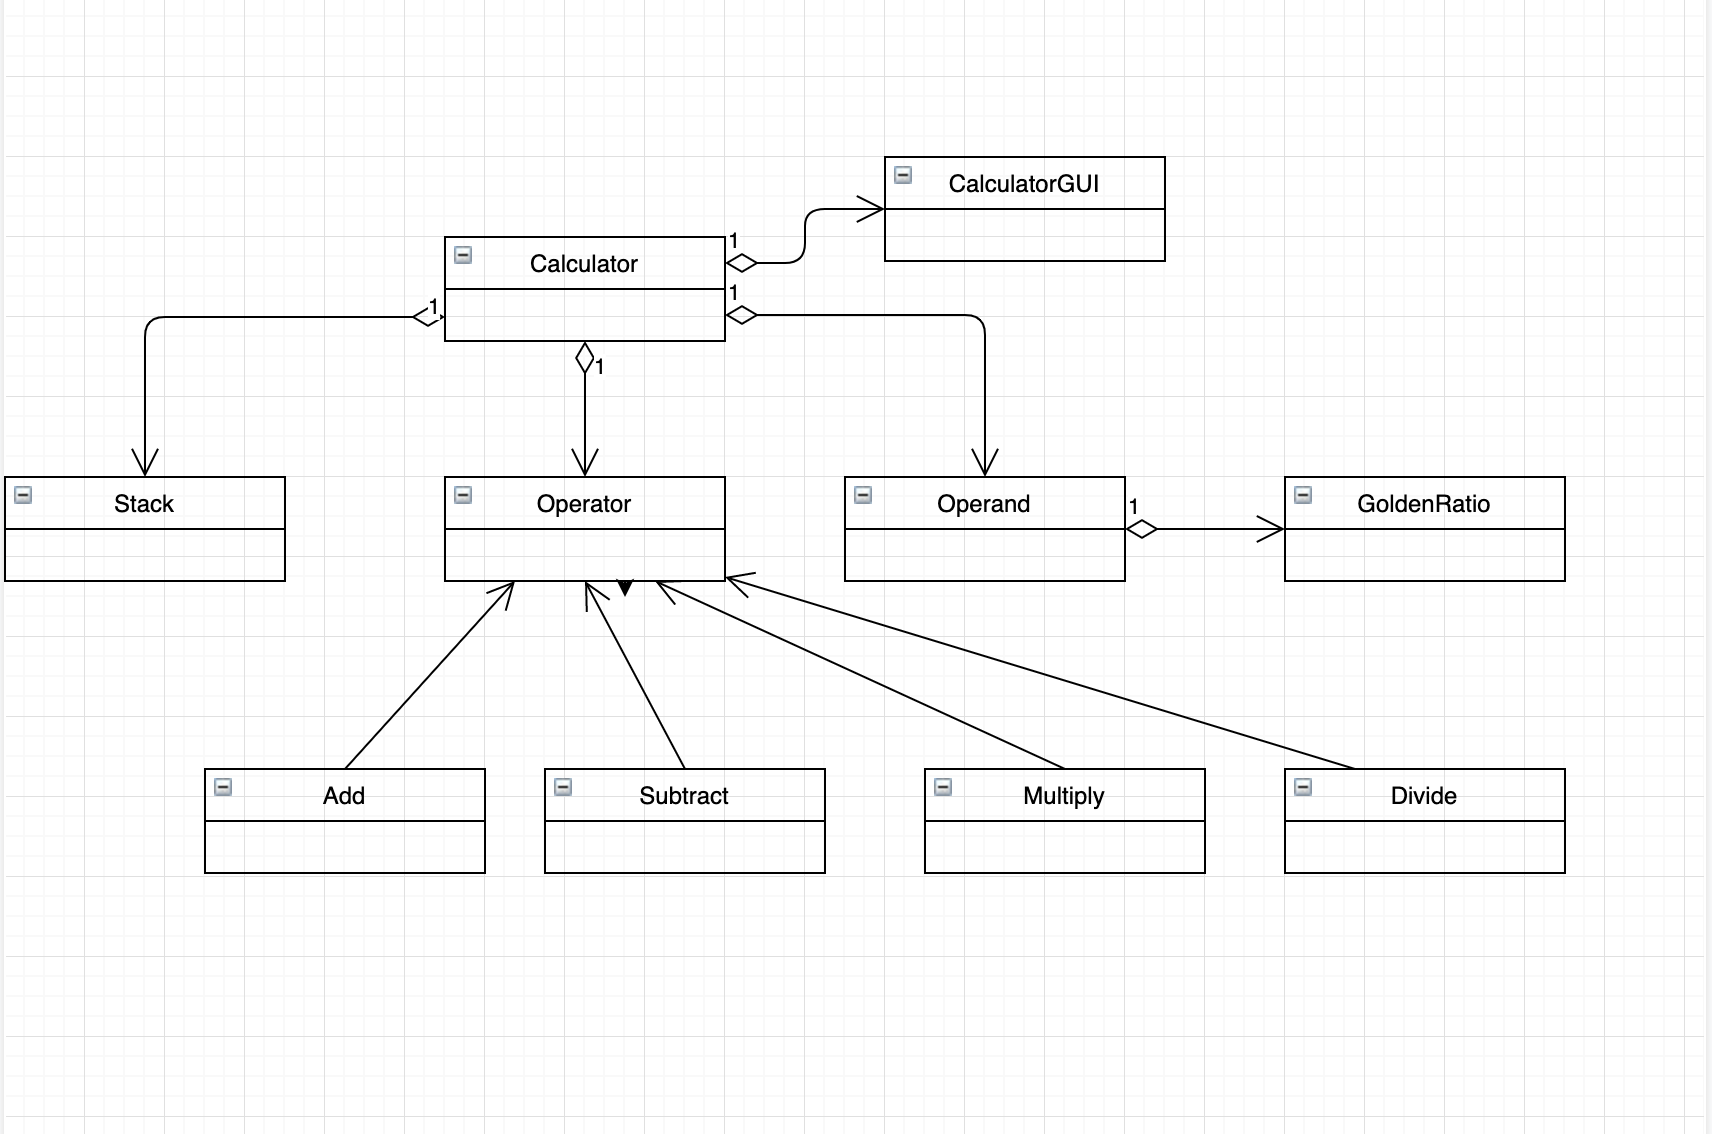
\includegraphics[width=1\textwidth]{domainmodel.png}
  \centering
  \caption{Domain Model}
\end{figure}



\newpage
\subsection{Domain Model Description}

\begin{table}[h]
\centering
\begin{tabular}{|l|l|}
\hline
\textbf{Concept Name} & \textbf{Calculator} \\
\hline

\textbf{Description} & \textbf{It is a basic calculator which takes input in GUI }\\
& \textbf{from user and looks for Operands and Operators.} \\
\hline
\end{tabular}
\end{table}


\begin{table}[h]
\centering
\begin{tabular}{|l|l|}
\hline
\textbf{Concept Name} & \textbf{CalculatorGUI} \\

\hline
\textbf{Description} & \textbf{It is Graphical User Interface.}\\ & \textbf{The user interacts with the GUI and gives inputs}\\
& \textbf{and it displays the output.}\\ & \textbf{It has aggregation relation with Calculator}\\
\hline
\end{tabular}
\end{table}


\begin{table}[h]
\centering
\begin{tabular}{|l|l|}
\hline
\textbf{Concept Name} & \textbf{Operator} \\
\hline
\textbf{Description} & \textbf{It is a class to identify the operators.}\\
& \textbf{It has aggregation relation with the calculator.} \\
\hline
\end{tabular}
\end{table}


\begin{table}[h]
\centering
\begin{tabular}{|l|l|}
\hline
\textbf{Concept Name} & \textbf{Golden Ratio} \\
\hline

\textbf{Description} & \textbf{It extends Operand and is an irrational number.}\\
& \textbf{The value is 1.618} 
\\
\hline
\end{tabular}
\end{table}
\newpage

\begin{table}[h]
\centering
\begin{tabular}{|l|l|}
\hline
\textbf{Concept Name} & \textbf{Addition, Subtraction, Multiply, Divide} \\
\hline

\textbf{Description} & \textbf{These extends the operator}\\
& \textbf{and add, subtract, multiply and divide operands}\\

\hline
\end{tabular}
\end{table}


\begin{table}[h]
\centering
\begin{tabular}{|l|l|}
\hline
\textbf{Concept Name} & \textbf{Stack} \\
\hline

\textbf{Description} & \textbf{It stores the numbers used and  the results}\\

\hline
\end{tabular}
\end{table}


\newpage
\section{Problem 5}
\subsection{Use Case Diagram}
\begin{figure}[htb!]
  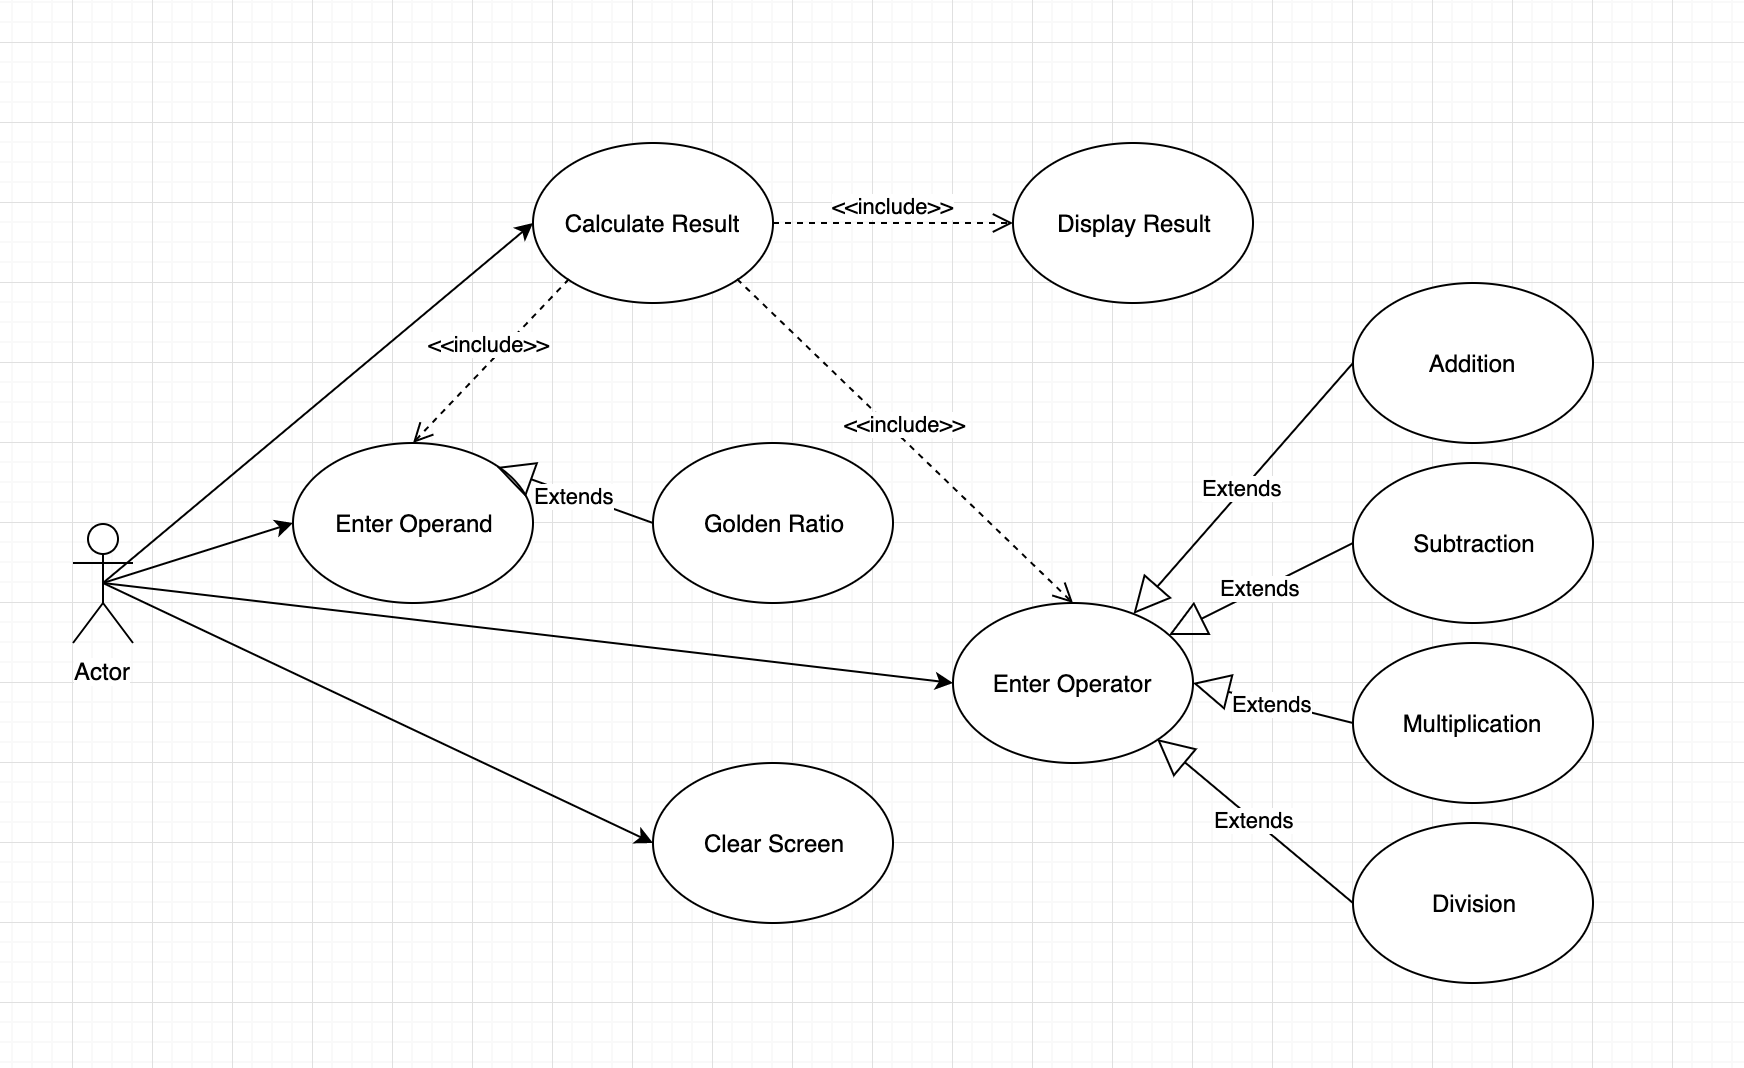
\includegraphics[width=1\textwidth]{Usecase.png}
  \centering
  \caption{Use Case diagram}
\end{figure}

\newpage
\subsection{Activity Diagram}

\begin{figure}[htb!]
  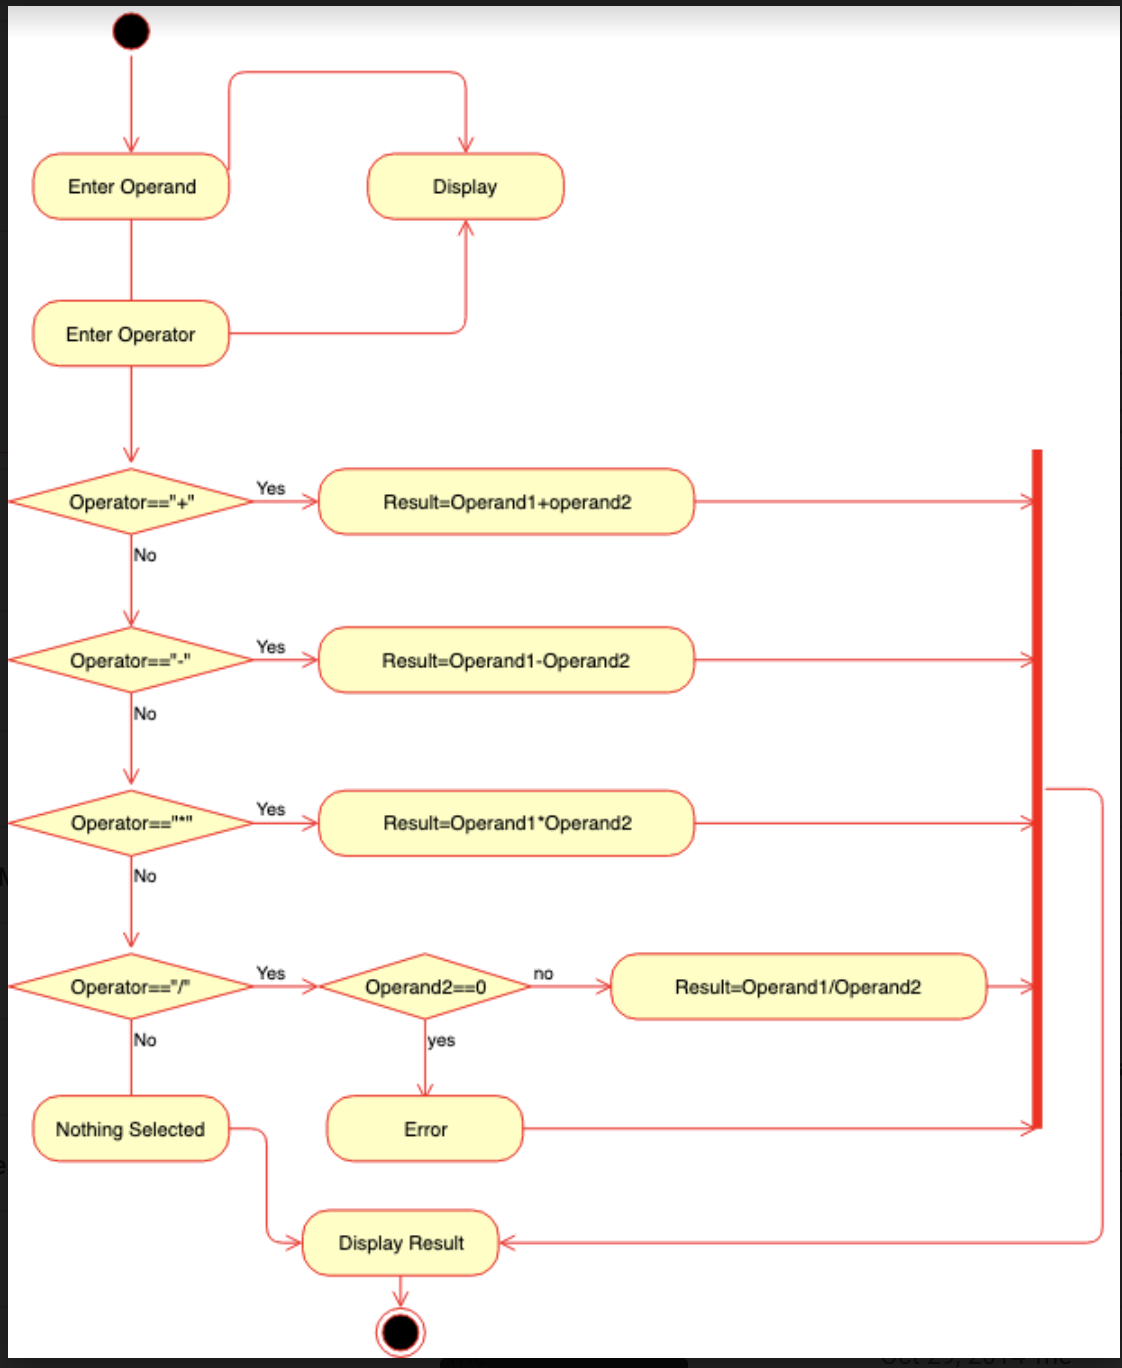
\includegraphics[width=1\textwidth]{activity.png}
  \centering
  \caption{Activity diagram}
\end{figure}

\newpage

\subsection{Scenario}

\begin{figure}[htb!]
  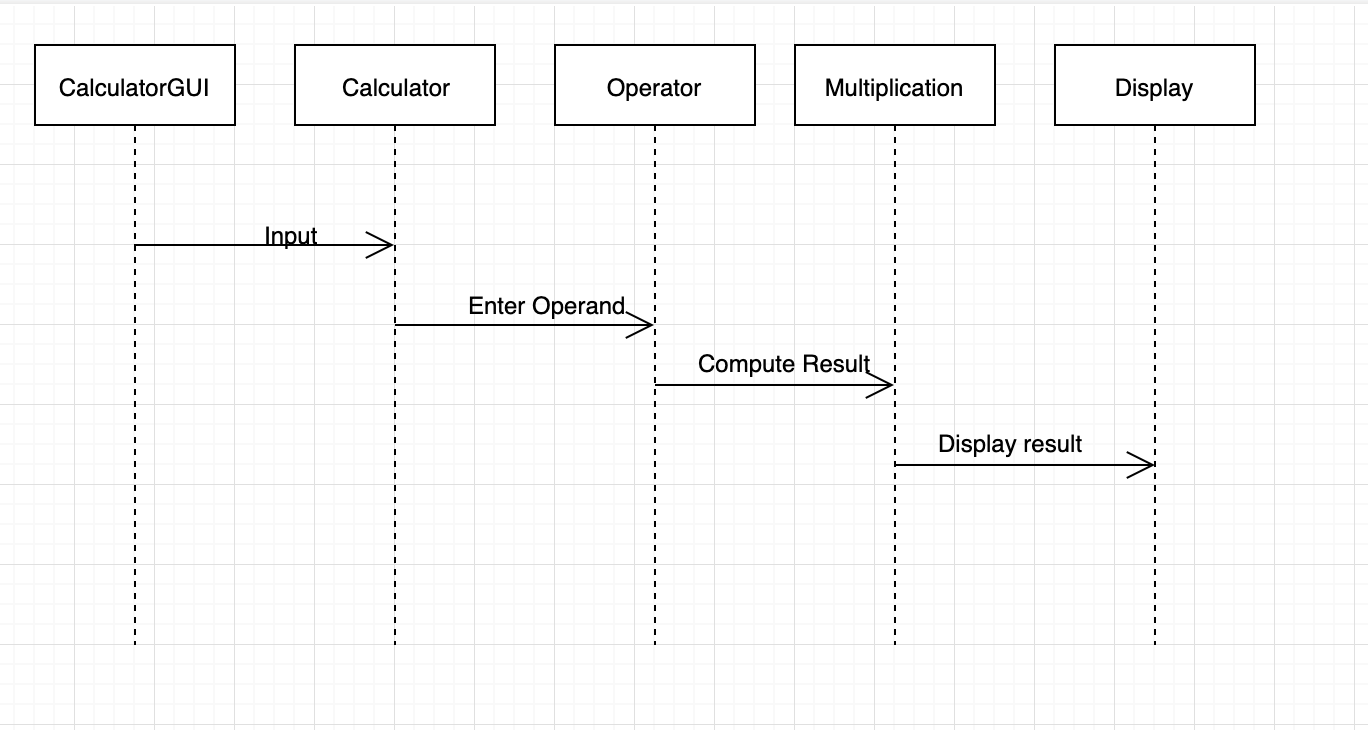
\includegraphics[width=1\textwidth]{sequencediagram.png}
  \centering
  \caption{Sequence Diagram}
\end{figure}

\begin{figure}[htb!]
  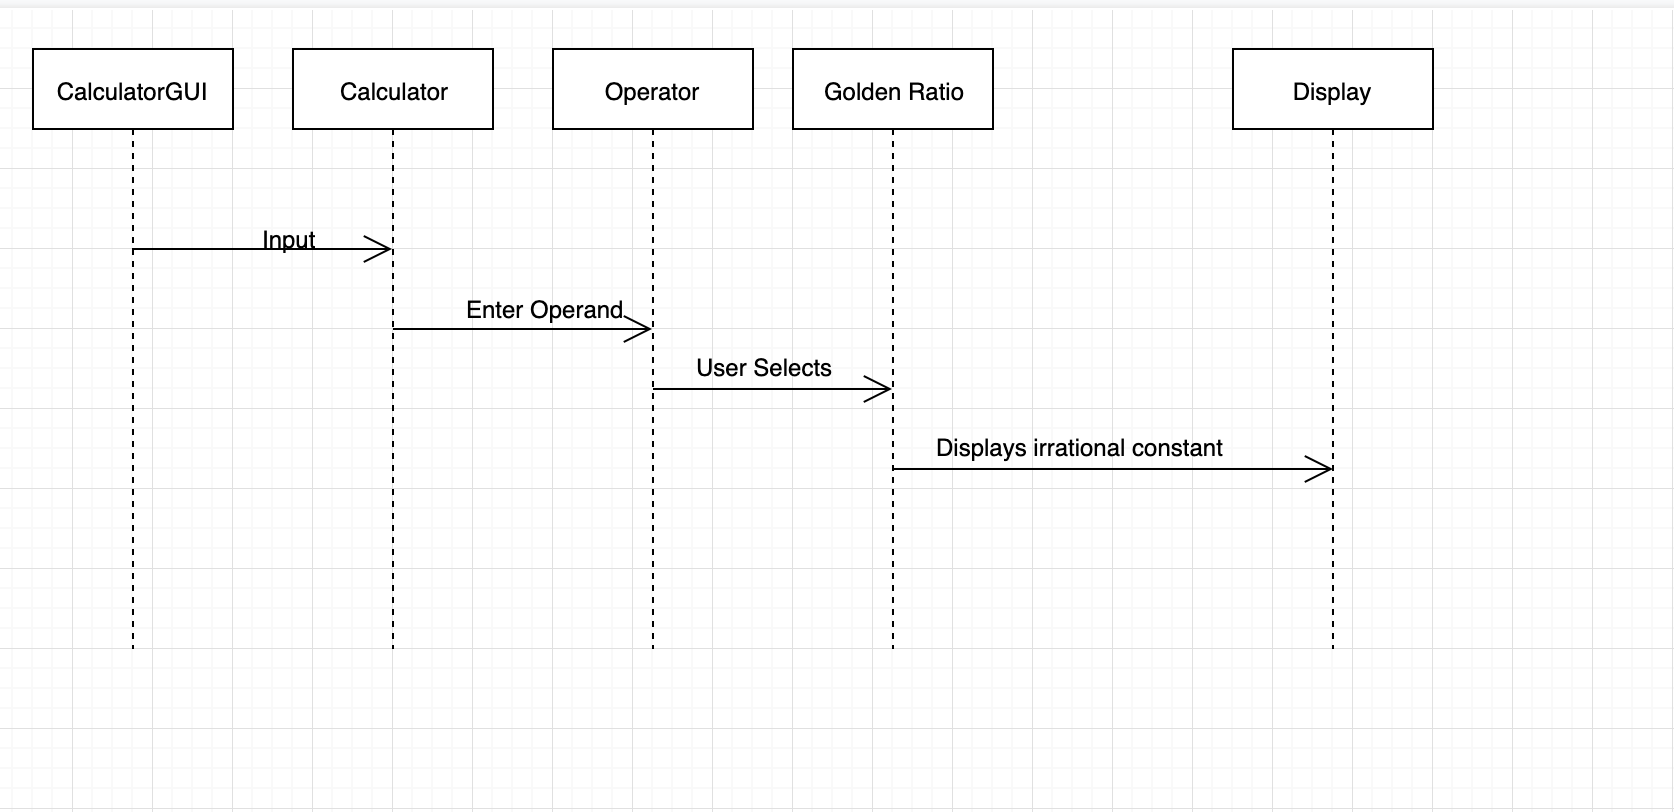
\includegraphics[width=1\textwidth]{scenario2.png}
  \centering
  \caption{Sequence Diagram with Golden Ratio}
\end{figure}

\newpage
\section{Problem 6}
\subsection{User Stories}
\begin{table}[h]
\centering
\begin{tabular}{|p{1cm}|p{6cm}|p{2cm}|p{2cm}|p{2cm}|}
\hline
\textbf{User} \textbf{Story}  & User Statement & Estimates & Constraints & Priority \\
\hline
US01 & \textbf{ The user can enter the shortest number}\textbf{ and obtain the largest number which } \textbf{satisfies Golden Ratio.} &  3 d & A $>$ 0 & HIGH\\
\hline
 US02 & \textbf{ The user can enter two positive operands} \textbf{and obtain the result of sum} \textbf{of these two.} & 1 d & A $>$ 0, B $>$ 0 & HIGH\\
\hline
 US03 & \textbf{ The user can enter two positive operands} \textbf{and obtain the result of subtraction} \textbf{of these two.}& 1 d & A $>$ 0, B $>$ 0  & HIGH \\
\hline
 US04 & \textbf{ The user can enter two positive operands and obtain the result of multiplication} & 1 d & A $>$ 0, B $>$ 0 & HIGH \\
\hline
 US05 & \textbf{ The user can enter two positive operands} \textbf{and obtain the result of division} & 1 d &  A $>$ 0, B $>$ 0 & HIGH\\
\hline
  US06 & \textbf{ The user can clear the screen for} \textbf{for entering new operands} & 1 d &  NONE & LOW\\
\hline

\end{tabular}
\end{table}
\newpage
\subsection{Acceptance Criteria for User Story}
1. User Story 1: When User enters one operand and then selects Golden Ratio, it will display a number larger than the operand which satisfies Golden Ratio.\newline
2. User Story 2: When User enter two operands and selects Operator Addition, it will display the result of the sum.\newline
3. User Story 3: When User enter two operands and selects Operator Subtraction, it will display the result of the subtraction.\newline
4. User Story 4: When User enter two operands and selects Operator Multiplication, it will display the result of the multiplication.\newline
5. User Story 5: When User enter two operands and selects Operator Division, it will display the result of the division.\newline
6. User Story 6: When User wants to clear the screen, it will clear the screen.\newline
\newpage
\section{Problem 7: Traceability Matrix}
\begin{table}[h]
\centering
\begin{tabular}{|p{2cm}|p{2cm}|p{6cm}|}
\hline
Number & User Story & Sources \\
\hline
1 & US01 & In Use Case diagram: Enter Operand, Golden Ratio \\
\hline
2 & US02 & In Use Case diagram:Enter Operator, Addition  \\
\hline
 3 & US03 & In Use Case diagram:Enter Operator, Subtraction \\
\hline
4 & US04 & In Use Case diagram:Enter Operator, Multiplication  \\
\hline
5 & US05 & In Use Case diagram:Enter Operator, Division\\
\hline
6 & US06 & In Use Case diagram:Clear Screen \\
\hline
\end{tabular}
\end{table}
\newpage

\begin{center}
    \textbf{Glossary}
\end{center}
Khinchin's constant-  For almost all real numbers x, coefficients ai of the continued fraction expansion of x have a finite geometric mean that is independent of the value of x and is known as Khinchin's constant.\newline\newline



\newpage
\bibliographystyle{plain}
\bibliography{M335}

\end{document}